Catchments were delineated using flow directions calculated with the eight-direction (D8) method on FABDEM reprojected to the UTM system, zone 19 south (WGS~84 datum), with \SI{30}{m} cells. A preliminary delineation in geographic coordinates underestimated the area. The outlet of each catchment is the cell with the greatest flow accumulation within \SI{120}{m} of the point where the mapped channel enters the urban development. The resulting areas are H1 with \SI{8.04}{km^2} and relief of \SI{1376}{m}, S1 with \SI{1.90}{km^2} and S2 with \SI{0.17}{km^2}: a total contributing area of \SI{10.1}{km^2}.

Two independent estimates were used, without combining them into a single distribution:
\begin{itemize}
\item \textbf{Rainfall--runoff balance with water and solids distinguished:} $V_w=f_wPAC$ and $V_m=V_w/(1-\Cvt)$, where $V_w$ is the water volume incorporated into the pulse; $P$, accumulated precipitation; $A$, catchment area; $C$, the runoff coefficient; $f_w$, the fraction of runoff incorporated into the pulse; and $V_m$, mixture volume. The ranges are: event-pulse precipitation $P$ between \SI{12}{\milli\metre} and \SI{35}{\milli\metre}, $C\in[0.3;0.8]$, $f_w\in[0.5;1]$ and $\Cvt\in[0.30;0.50]$.
\item \textbf{Empirical model for burned catchments} \citep{gartner2014}, applied by subcatchment and including its residual error $\varepsilon\sim N(0;1.04^2)$. This model predicts deposit volume $V_\mathrm{dep}$, which is converted to mixture volume using $V_m=(1-\phi)V_\mathrm{dep}/\Cvt$, where $\phi$ is deposit porosity. Its applicability outside southern California is a hypothesis.
\end{itemize}
The distributions are summarized by the median and the 5th and 95th percentiles, and the corresponding peak discharge is estimated using the relationship of \citet{mizuyama1992}. Calibration spans volumes from \SI{80000}{\metre\cubed} to \SI{300000}{\metre\cubed}. Initial results are presented in Section~\ref{sec:res-volumen}; the update with severity estimated by dNBR is presented in Section~\ref{sec:res-incendio}.

\begin{figure}[htbp]\centering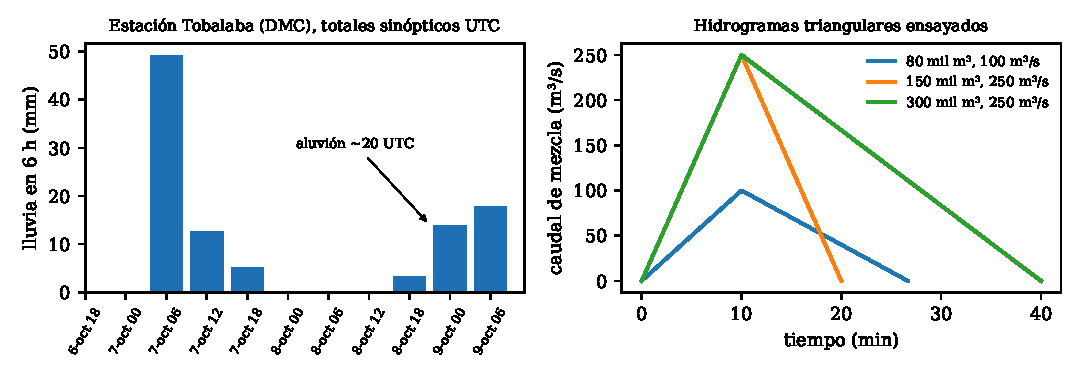
\includegraphics[width=\textwidth]{forzamiento}\caption{Observed and assumed model forcing. Left: rainfall accumulated over \SI{6}{h} intervals at the Tobalaba station of Dirección Meteorológica de Chile \citep{dmc2026} between 6 and 9 October 2026 (UTC times; the press reports cited in the account place the debris flow at about 20 UTC on 8 October). Right: triangular mixture hydrographs tested.}\label{fig:forzamiento}\end{figure}

\paragraph{Saturated-Soil Scenario.} With the hydrometeorological information obtained after screening (Section~\ref{sec:evidencia}), a third estimate was added, also without combining it with the previous ones. The relationship between the reported isotherm and the maximum catchment elevation (\SI{2355}{m}, the same as reported by CR2; an earlier version of the text mistakenly stated \SI{2775}{m}, a figure not used in any calculation: D8 delineation and hypsometry were always based on the elevation model) supports the assumption of liquid precipitation over the entire contributing area, and the soil saturation reported by the authority is adopted as an assumption of the calculation scenario. The ranges used are $P\in[20;40]$~\si{mm}, $C\in[0.6;0.9]$ and $f_w\in[0.6;1]$. The snowmelt contribution is bounded above by \SI{50}{mm} water equivalent over the \SI{0.31}{km^2} of the catchment above \SI{2000}{m}.
